\chapter{Introduction}
\pagenumbering{arabic}
\setcounter{page}{1}
\section{Background}
The Norwegian economy is cooling under a pessimistic oil price of close to 45 USD per barrel as of autumn 2015. Under heavy pressure to perform, companies involved in the exploitation of hydrocarbons are cutting costs while trying to increase productivity.

As a means of improving profitability, decision support systems have been developed, which tries to provide real-time support when drilling oil wells. One example of these was a product of work done at NTNU.

A roadmap for automating drilling systems was established in June 2013 with the objective of providing a guideline to the future emergence of drilling systems automation.

Automation of pipe handling have been pursued by several companies in the oil rig equipment production market with moderate success. The industry have realized that more may be gained from supporting humans in the center of the operation, than to completely eliminate humans. As such, systems to support the human driller need to be developed.

Support systems that may improve safety and productivity includes improvements to the graphical user interface, presentation of relevant and aggrevated data, as well as integrated camera systems.

The main objective of this MSc thesis is to implement a system that provides a better situation overview through automated CCTV tracking of machines.

This MSc thesis should address the following:
\begin{itemize}
\item Implementation of an auto tracking CCTV system using glyphs as visual descriptor.
\item Analysis of dataset with real-world weather over a long period.
\item Prototyping of an algorithm to detect casings and pipes in a fingerboard.
\end{itemize}

\subsection{Problem formulation}
How can computer vision assisted camera tracking be exploited to increase safety and situational awareness in any process involving heavy machinery and remote operation?

How will GPU-acceleration of the computer vision algorithm affect the system?

How can we reduce the latency of the live camera feed to make feedback control of the camera better?

How can we track an object across multiple cameras?

We will develop a solution to provide benefits to a human driller operating heavy machinery on an oil rig, but the solution is not limited to this application. Our end goal is to reduce the possibility of an undesired event, be it either damage to humans or expensive equipment.

\subsection{Literature survey}
As discussed by \citet{sklet05}, the concept of a safety barrier is not clearly defined and its meaning is ambiguous. With this in mind, we are looking to implement what \citet{rausand14} describes as a proactive safety barrier, also known as a frequency-reducing barrier, in other words a system to reduce the frequency of undesired events.

Semi-automated CCTV surveillance have been considered by \citet{dadashi12} as a method of increasing the capacity of a human operator in a traditional human surveillance situation. The reliability for fully automated systems were not considered good enough for an operator to trust. The findings recommend providing feedback about system confidence and accuracy to the operator, which makes the automated component of such a system more 'visible' to its user. For the case of this thesis, the act of displaying visual cues overlaid on the CCTV images are considered. This would hopefully increase trust, and expose the automated component of our fully automated tracking system.

The machine vision algorithm that was implemented in the authors earlier work, as mentioned in work done by \citet{boyers13} and \citet{kirillov10}, will be used to recognize the distinct symbol, hereafter called a glyph.

Our camera of choice, an AXIS Q6045 was selected both by its widespread use in the oil- and gas industry, and because this is what the author had at hand. It is a modern high-definition PTZ-camera produced by Axis Communications.  Axis Communications have provided a white paper which provides a good overview of the various elements that increase latency in a live video stream. This document is available online. \citep{axis15}

The inherit differences between analog and digital video transmission have been examined by \citet{hill10}, and the conclusion was that latency present in digital transmission is approaching negligible for normal usage. Still, the article presents findings that show latency of a digital transmission being more than 5x of the analog transmission latency. The upsides of digital transmission include increased quality of image, flexibility of digital encoding and ability to use analytic software.

Work done by \citet{svensson13} involved methods to reduce the delays that are inherently found in digital video transmission systems and the control of these. Their research was done on AXIS Q6035 and AXIS Q6032 cameras. The author assumes these to be closely related to the AXIS Q6045, and their findings therefore useful for work done in this thesis. Findings include camera firmware being among the key factors for video delay, as the stock cameras have implemented an inefficient communication scheme, and there are other suggestions to reduce delay presented. For the scope of this thesis, we will have these delays in mind and build around them, as any firmware upgrades have to come from Axis themselves if any company would consider using them.

Tracking of objects across multiple cameras have been explored with most focus on overlapping camera views. Some work has also been done on non-overlapping camera views by \citet{javed03}, where camera topology and path probabilities are learnt without any inter-camera calibration. As soon as one uses images from several sources, the timestamp for the images becomes crucial as a point of reference. Through the use of Parzen windows, the inter-camera space-time probabilities can be mapped. The method mentioned does require a learning phase.

\subsection{What remains to be done?}
As a summary of the literature survey, we see that much work has been done in the different fields, but not much have been found on combining the results of these into a solution that can provide modern, automated CCTV tracking of industrial processes involving heavy machinery in a way that retains the human operator in the center of the process.

We aim to break down the information silo and combine as much as possible, given constraints of time, into a proof of concept which can be the stepping stone to a commercial product.

\section{Objectives}
The objectives of the work done through this thesis consists of:
\begin{enumerate}
  \item Implementation of a multi-source GPU-accelerated machine vision program that can control a CCTV camera and follow a symbol
  \item Implementation of a proof of concept pipe-detection algorithm for fingerboards
\end{enumerate}

\section{Limitations}
The limitations that relates to this study includes both technical challenges, environmental and operational conditions as well as oil politics in a broad sense, but focus is on the technical challenges for the sake of brevity.

As CCTV cameras have evolved, the video transfer method has gone through some changes to cater for higher resolution and more true representation of the world as observed. By this, analog signals have been replaced by digital signals. Analog transmission is known for being both robust, simple and near-instant, however they are prone to signal deterioration which may affect machine vision algorithms, and their flexibility of location is not as good as modern digital transmission. With digital transmission, usually over Ethernet, the cost of these systems have gone down, flexibility have gone up and resolution as well as control has improved, yet this have introduced new challenges. Data loss is a real possibility, increased latency through encoding and decoding of the video stream and a shared network highway puts more demand on the implementation. One serious limitation to the implementation of the system as presented, is therefore as a feedback system, the upper latency limit for which when the system becomes unstable.

The oil industry is considered a conservative one, as lost production time can lead to extreme expenses and questions regarding responsibility and passing on cost to service providers. Technology is also highly guarded, as the sheer amount of money that can be gained from saving a fraction of time, means that cooperation is not common in the industry, and transparency of systems and solutions may be less than ideal. The idea then, of making changes to what already works, is not easy to plant, and this also limits the available data set for the purpose of making robust systems.

Heterogeneous computing platforms are still considered to be in its infancy, and both CUDA as well as OpenCL is under active developement. Choosing one technology will lead to an exclusion of either benefits or available computing platforms. A limitation here is that the resulting speed and benefits of heterogeneous computing are not set in stone, and that there will always be improvements that can be done to make an otherwise unworkable system to a brilliant idea.

The software world progress quickly, and new solutions can suddenly become obsolete, requiring legacy maintenance and making in-house developed software seem much like building a tower of cards as the flux of developers who knows the system changes over time. This would make an externally maintained solution seem like a better idea, but sharing information to make the development work is not an easy task as each company protects its own interests.

It is considered a hard challenge therefore, to make a truly reliable system that works in the real world. Making a tabletop solution is not nearly enough to allow a big company to test this out in the real world.

Seeing past these limitations, however, is a world of possibilities, which this study tries to explore.

\section{Approach}
\subsection{CCTV tracking system}
The implementation of the CCTV tracking system will be based on the authors previous work and be written in C++ with heterogeneous support from a GPU to increase performance.

After this system has been built, it will be tested with and without GPU acceleration, to determine if the full solution becomes more stable and reliable.

A data-set will be analyzed to test the robustness of the machine vision algorithm and comment how snow, sun and other real-world factors affect the output.

It will also be tried to use multiple video sources, however due to the lack of several CCTV cameras, this will only partially be explored using a common webcamera, as a means of doing camera handover.

\subsection{Pipe detection system}
The construction of a proof of concept pipe detection system for fingerboards will be done in a rapid prototyping environment, to show that it is possible to increase control system awareness in existing infrastructure on the oil rig.

\section{Structure of the report}
Some diagrams have been made by the author. These diagrams follow a coloring scheme, to ease reading.

\begin{figure}[ht]
    \centering
    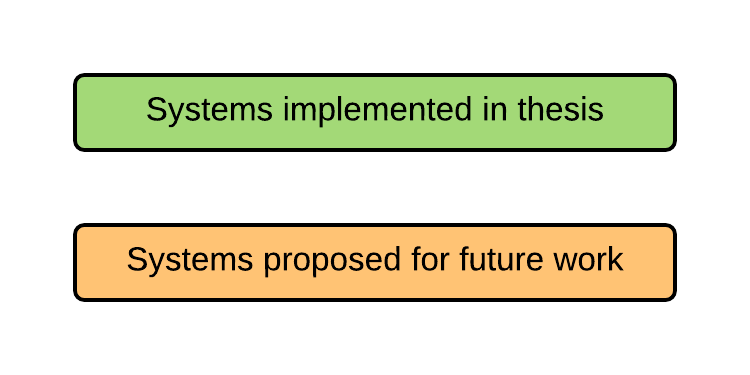
\includegraphics[width=0.8\textwidth]{coloring.png}
    \caption{Color scheme for diagrams. Source: Own work}
    \label{fig:coloring}
\end{figure}
\FloatBarrier

The colors of boxes are used to describe their role in the total picture. See figure \ref{fig:coloring} for a description of their function.
All the software developed as a part of this project can be found at the authors personal repository at Github ~\cite{github}, feel free to use this for future non-commercial work. The Latex source is also available.

\section{Structure of the DVD}
The DVD contains a snapshot of the latest Github code repository as of the date of this report.